\documentclass{beamer}
\usetheme{Boadilla} % Clean structure
\useinnertheme{circles} % Dots for sections
\useoutertheme{miniframes} % Header nav with section progress
\setbeamertemplate{navigation symbols}{} % Remove nav icons

\usepackage[utf8]{inputenc}
\usepackage{amsmath, amsfonts, graphicx, booktabs, hyperref}
\usepackage{tikz, caption}

% Custom colors
\definecolor{DeepBlue}{RGB}{0,51,102}
\setbeamercolor{title}{fg=DeepBlue}
\setbeamercolor{frametitle}{fg=DeepBlue}
\setbeamercolor{structure}{fg=DeepBlue}
\setbeamercolor{item}{fg=DeepBlue}

% Frame title underline
\setbeamertemplate{frametitle}{
    \insertframetitle\\
    \vspace{-0.3cm}
    \color{DeepBlue}\rule{\linewidth}{0.2mm}
    \vspace{0.3cm}
}

% Footer with long title and date
\setbeamertemplate{footline}
{
  \leavevmode%
  \hbox{%
  \begin{beamercolorbox}[wd=.20\paperwidth,ht=2.25ex,dp=1ex,center]{author in head/foot}%
    {\fontsize{6}{6} \selectfont Anushka Mukherjee}
  \end{beamercolorbox}%
  \begin{beamercolorbox}[wd=.60\paperwidth,ht=2.25ex,dp=1ex,center]{title in head/foot}%
    \usebeamerfont{title in head/foot}{\fontsize{6}{6}\selectfont Modeling Household Carbon Footprints - August 19, 2025}
  \end{beamercolorbox}%
  \begin{beamercolorbox}[wd=.20\paperwidth,ht=2.25ex,dp=1ex,right]{date in head/foot}%
    {\fontsize{6}{6} \selectfont \insertframenumber{} / \inserttotalframenumber}\hspace*{1em}
  \end{beamercolorbox}}%
  \vskip0pt%
}

% Title info
\title[Modeling Household Carbon Footprints]{Modeling Household Carbon Footprints: Methods, Metrics, and Estimation Frameworks}
\author[Anushka Mukherjee]{Anushka Mukherjee\\Matriculation No: 50075072}
\institute[University of Bonn]{University of Bonn}
\date[July 2025]{Master's Thesis Presentation\\August 19, 2025}

\begin{document}

% Title slide
\begin{frame}
  \titlepage
\end{frame}

% Table of contents
\begin{frame}{Overview}
  \tableofcontents
\end{frame}

% -------------------
\section{Introduction}
\begin{frame}{Motivation}
\vspace{-1.5em}
\small
Households are increasingly recognized as key actors in climate mitigation. However, the methods used to estimate their carbon footprints differ widely.

\begin{columns}
  \begin{column}{0.65\textwidth}
    \begin{itemize}
      \item Existing tools:
      \begin{itemize}
        \item Apply divergent system boundaries  (e.g., direct vs. full life-cycle emissions)
        \item Often double-count emissions 
        \item Fail to account for market feedback or investment-related emissions
      \end{itemize}
    \end{itemize}
  \end{column}
  \begin{column}{0.2\textwidth}
    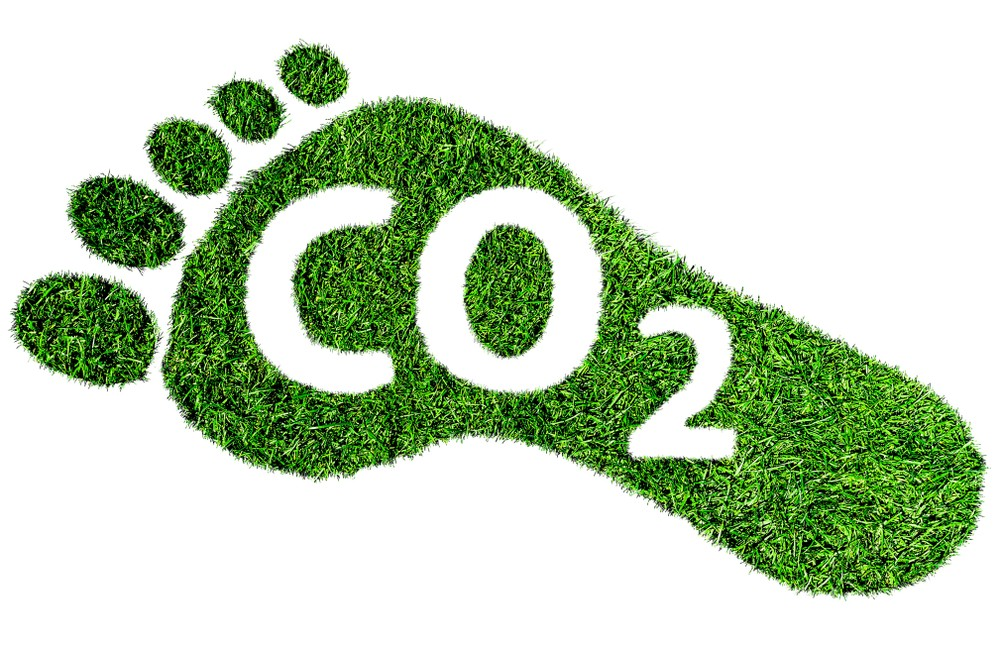
\includegraphics[width=\linewidth]{co2.jpg}
  \end{column}
\end{columns}

\vspace{1em}
\begin{itemize}
\item \small \textbf{Analytical Problem}: The attribution logic embedded in each method fundamentally shapes how household responsibility is quantified.\\
\item \small \textbf{Research Gap}: No unified framework currently compares GHG Protocol, LCA, EEIO, and general equilibrium models from a responsibility perspective.\\
\item \small \textbf{Contribution}: This thesis systematically compares four models to assess attribution differences, empirical consequences, and policy alignment.
\end{itemize}
\end{frame}



% -------------------
\section{Research Questions and Methodology}
\begin{frame}{Research Questions}
\begin{enumerate}
  \item How do footprint estimates vary across models?
  \item How is household responsibility estimated and attributed under each carbon accounting method?
  \item How do attribution methods shape policy and equity outcomes?
\end{enumerate}
\end{frame}

\begin{frame}{Methodology (I): Analytical Framework}
\small
\vspace{-2.0em}
\begin{itemize}
  \item A comparative framework is used to analyze how different carbon accounting methods attribute household emissions.
  \item The analysis covers four dominant models:
  \begin{itemize}
    \item \textbf{GHG Protocol (Production-based):} Focuses on direct household emissions (Scopes 1–2)
    \item \textbf{Life Cycle Assessment (Product-based):} Attributes emissions across a product's lifecycle
    \item \textbf{EEIO Model (Consumption-based):} Traces emissions through upstream production based on household expenditure
    \item \textbf{Hakenes–Schliephake Model (Consequentialist):} Assigns responsibility based on marginal impact in general equilibrium framework
  \end{itemize}
  \item For each method, the attribution logic, model assumptions, and policy outcomes are compared.
\end{itemize}
\end{frame}

\begin{frame}{Methodology (II): Addressing the Research Questions}
\vspace{-2.5em}
    \small
\textbf{Research Questions Addressed}
\small
\begin{enumerate}[$\Rightarrow$]
  \item \textbf{RQ1:} How do footprint estimates vary across methods?
  \begin{itemize}
    \item Empirical illustrations are derived using official household expenditure data (Eurostat, USDA) and publicly available emission factors (EXIOBASE, Climatiq, IPCC).
    %\item Each method is applied to a harmonized dataset for France, Spain, Germany, and the U.S. wheat sector.
  \end{itemize}
  \item \textbf{RQ2:} How does each method attribute household responsibility?
  \begin{itemize}
    \item Theoretical derivations and decomposition techniques illustrate attribution logic and scope.
    \item Attribution is classified as operational, consumption-based, or consequentialist.
  \end{itemize}
  \item \textbf{RQ3:} What are the equity and policy implications?
  \begin{itemize}
    \item Each attribution model is linked to relevant policy instruments and their distributional impacts.
  \end{itemize}
\end{enumerate}
\end{frame}

\section{Literature Review}
\begin{frame}{Literature Review: Evolution of HCF Estimation}
\small
\vspace{-2.5em}
\begin{itemize}
  \item Research on household carbon footprints (HCF) has expanded since the early 2000s, evolving across three broad phases:
  \begin{itemize}
    \footnotesize
    \item \textbf{Early phase:} IO-based estimation of emissions by expenditure category (Pachauri \& Spreng, 2002; Lenzen, 2004)
    \item \textbf{Expansion:} National comparisons and household heterogeneity (Druckman \& Jackson, 2009; Baiocchi \& Minx, 2010)
    \item \textbf{Integration:} Inequality, global supply chains, and lifestyle effects (Ivanova et al., 2015; Moran et al., 2018)
  \end{itemize}

  \item Dominant methods in current literature:
 
  \begin{itemize}
    \item  \footnotesize \textbf{GHG Protocol:} Activity-based, scope-defined inventories (IPCC Guidelines, 2019)
     \item \footnotesize \textbf{LCA:} Process-based alternative, tracing cradle-to-grave emissions (Steubing et al., 2022)
     \item \footnotesize \textbf{EEIO:} Economy-wide linkages via input–output matrices (Baiocchi \& Minx; 2010, Wiedmann, 2009)
     \item \footnotesize \textbf{GE Models:} Endogenizes household decisions and emissions via market-clearing and investment feedback. (Hakenes \& Schliephake, 2024)
  \end{itemize}
\end{itemize}
\end{frame}


\begin{frame}{Literature Review: Publication Trends and Focus Areas}
\small
\vspace{-2.5em}
\begin{itemize}
  \footnotesize
  \item A bibliometric analysis of \textbf{1,311 peer-reviewed articles (2000–2025)} shows a sharp rise post-2015 (Paris Agreement).
  \item Research is concentrated around \textit{input–output analysis, sustainable consumption}, and \textit{life cycle assessment}.
  \end{itemize}
\vspace{-1.0em}
\begin{columns}
  \centering
  \begin{column}{0.5\textwidth}
    \centering
    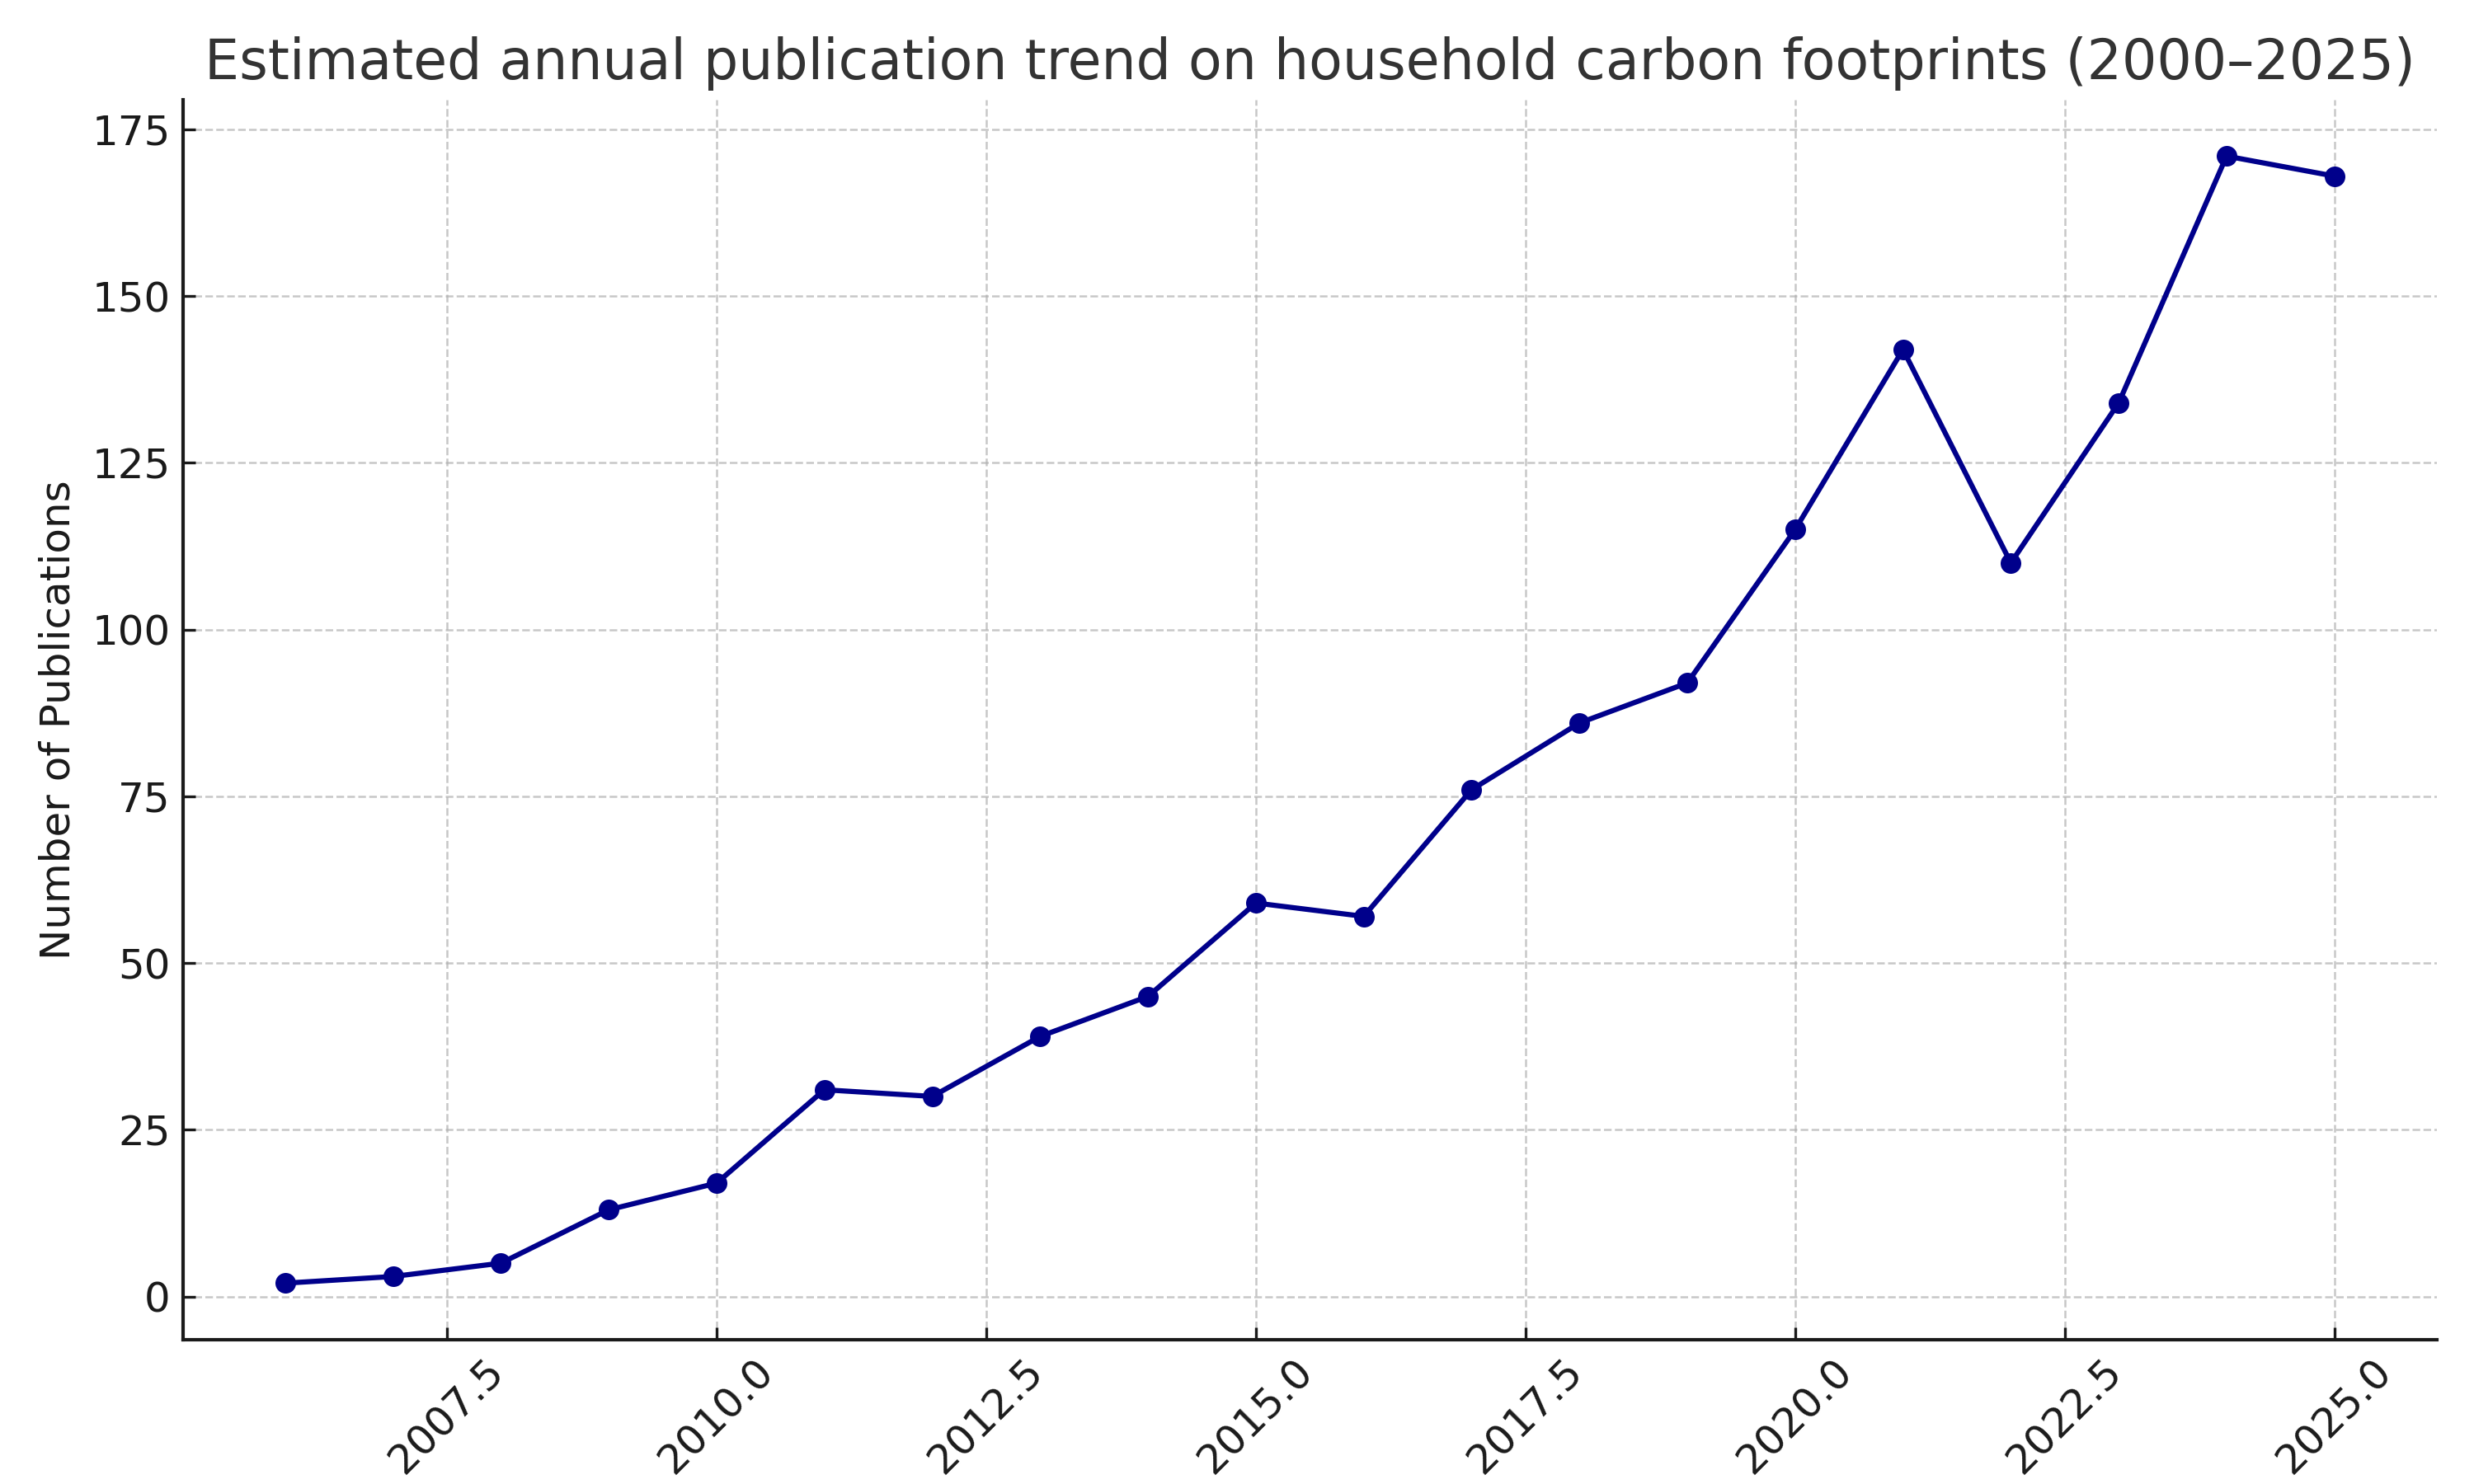
\includegraphics[width=0.8\linewidth]{publication_trend_darkblue_estimated2025.png}
  \end{column}
  \begin{column}{0.6\textwidth}
    \centering
    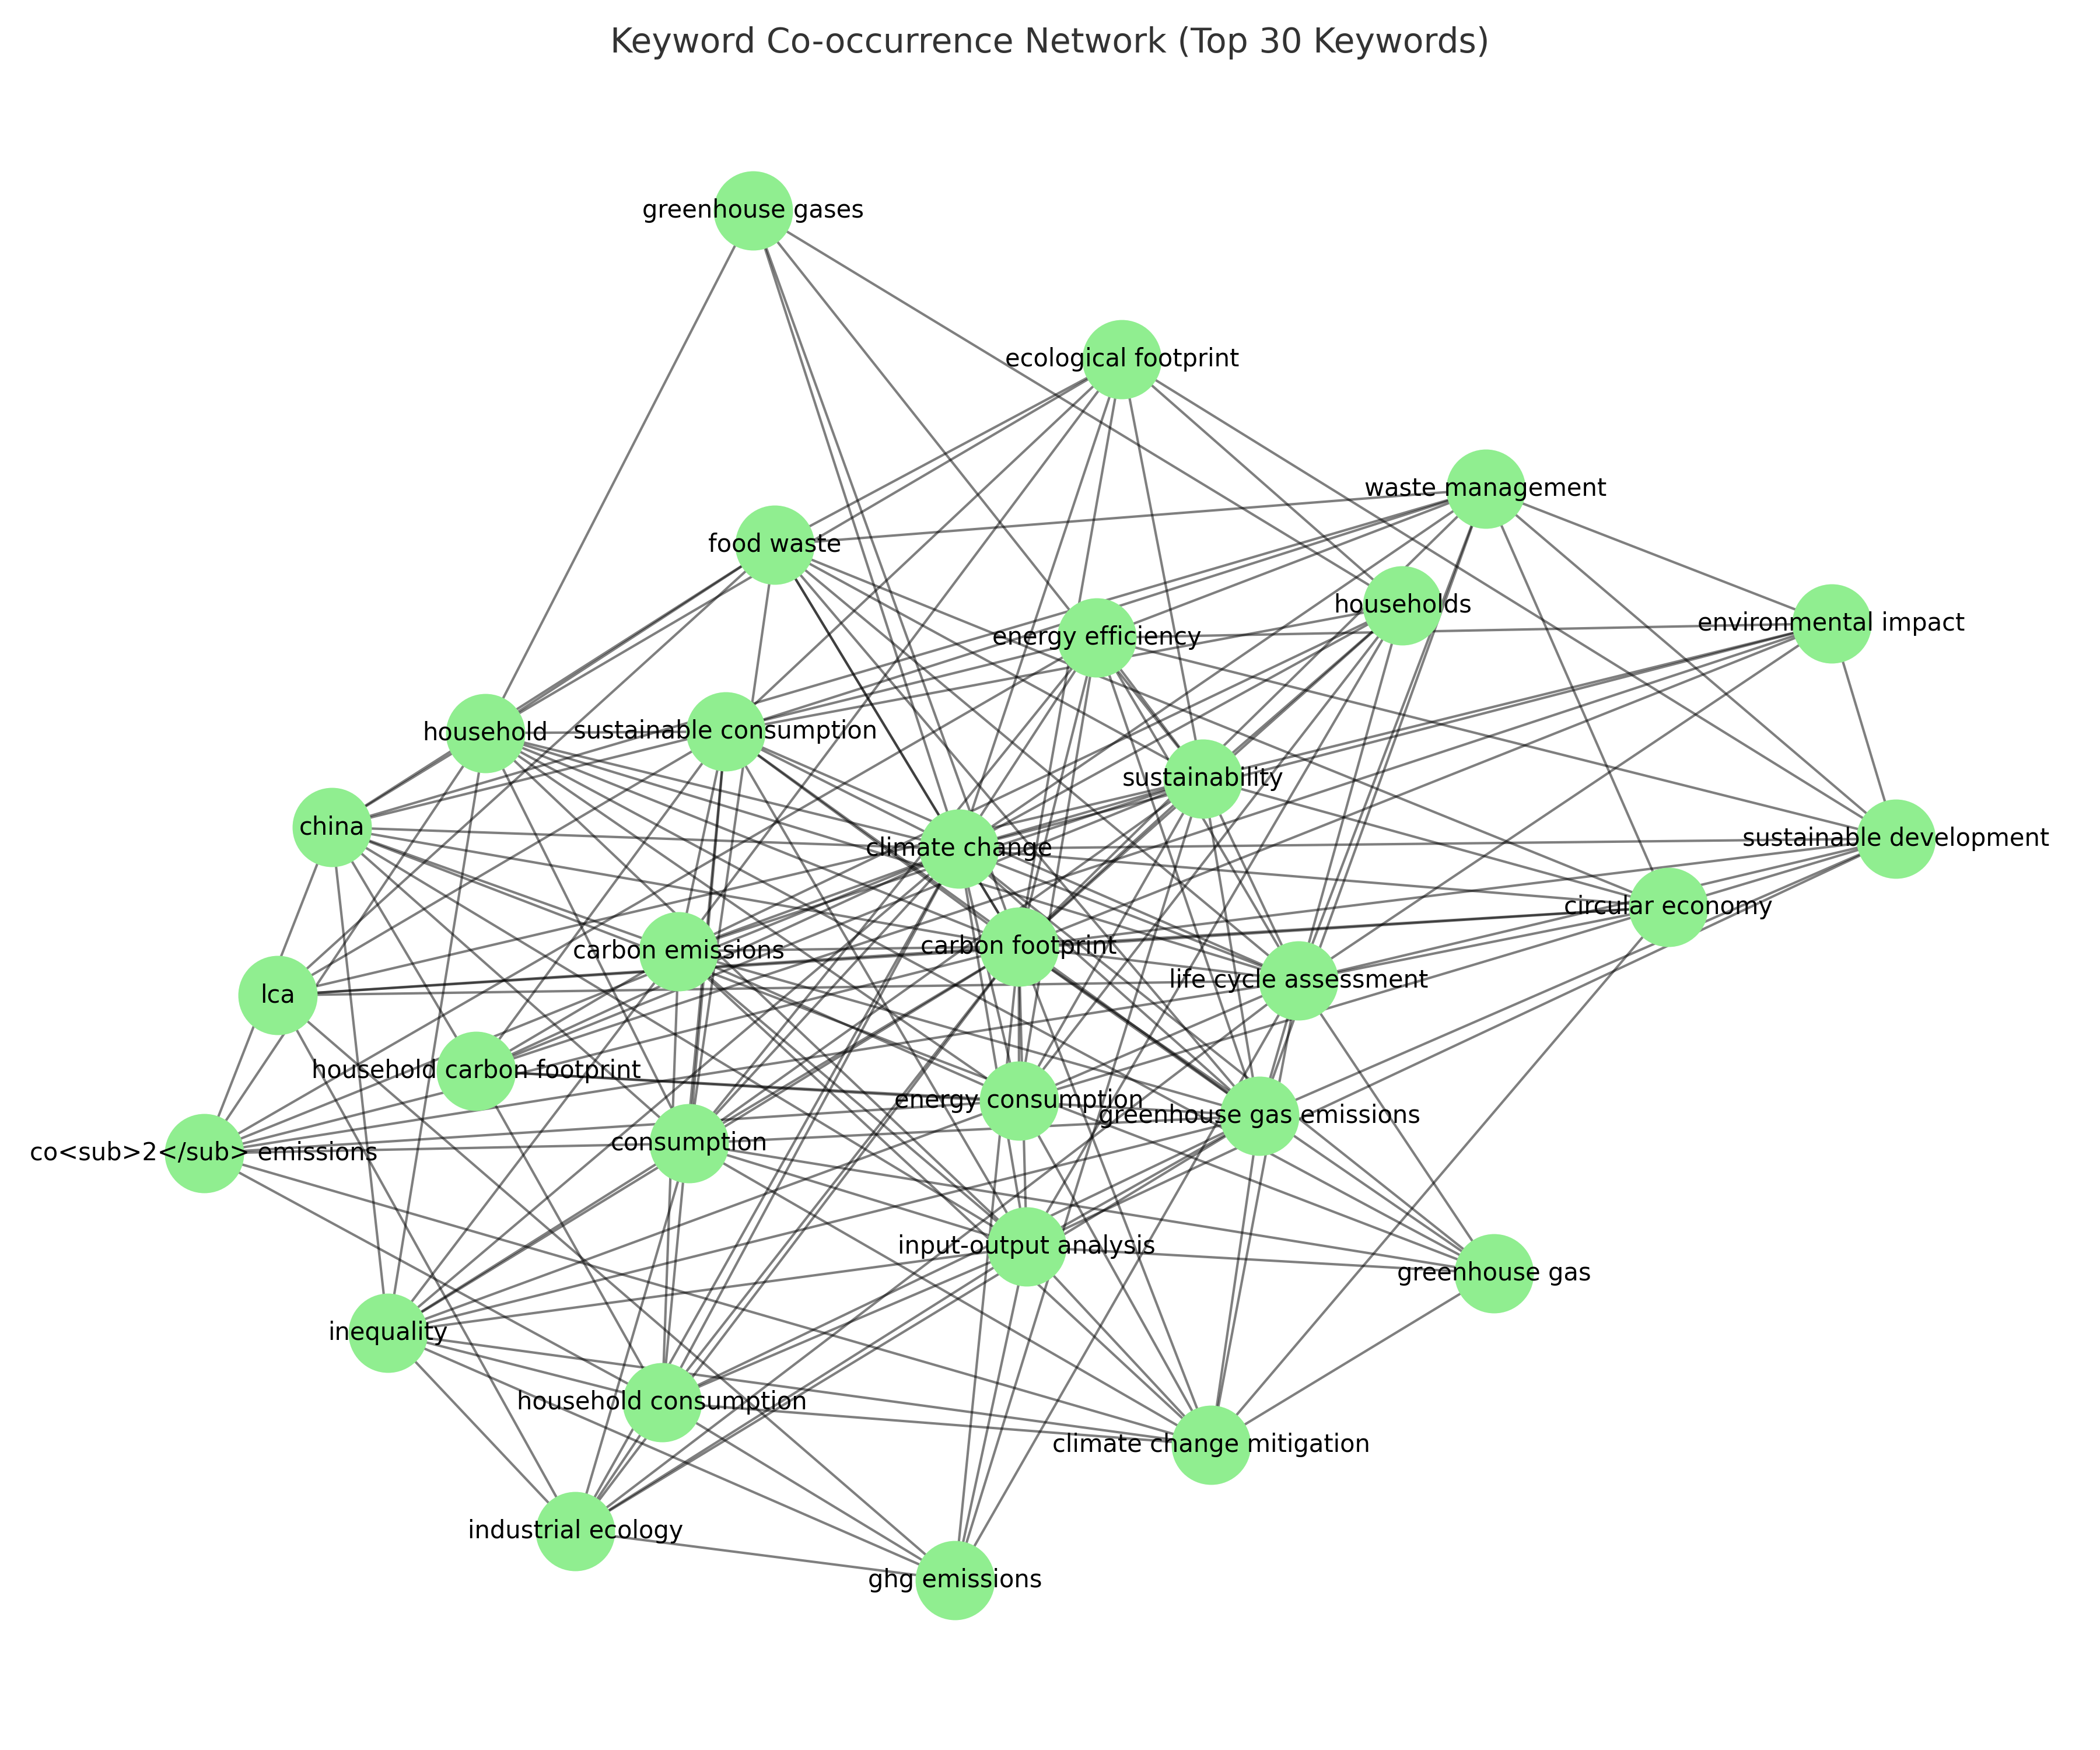
\includegraphics[width=0.7\linewidth]{keyword_cooccurrence.png}
  \end{column}
\end{columns}

\vspace{-0.5em}
\begin{itemize}
  \footnotesize
\item Top Journals: \textit{Journal of Cleaner Production}, \textit{Science of the Total Environment}, and \textit{Environmental Science \& Technology}
  \item Top institutions: University of Tokyo, Sun Yat-sen University, University of Maryland.
\end{itemize}

\end{frame}

\begin{frame}{GHG Protocol: Emission Inventory Framework}
\small
\vspace{-2.5em}

\footnotesize \textbf{Definition:}  
The Greenhouse Gas (GHG) Protocol is a standardized framework developed by WRI and WBCSD for tracking emissions across three scopes.
\vspace{-0.5em}
\begin{figure}[h]
  \centering
  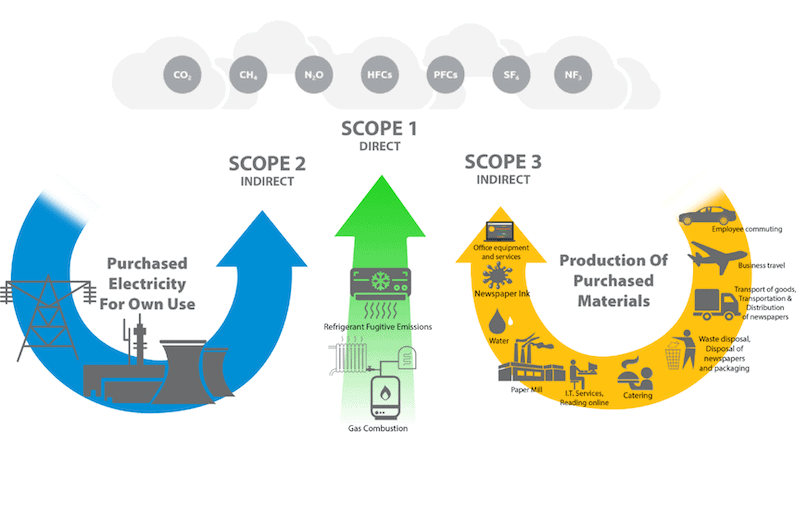
\includegraphics[width=0.55\linewidth]{ghg scope.png}
  \caption*{\tiny Source: Green Element (2023) — https://greenelement.co.uk}
\end{figure}
\vspace{-1.0em}
\footnotesize \textbf{Formulation:}
\[
\text{CF}_{\text{household}} = E_{\text{Scope 1}} + E_{\text{Scope 2}} + E_{\text{Scope 3}}, \quad 
E_i = \sum_j Q_{ij} \cdot EF_{ij}
\]
{\footnotesize where $Q_{ij}$ is the activity level and $EF_{ij}$ is the emission factor for activity $j$ under scope $i$.}

\end{frame}

\section{Methods and Applications}

\begin{frame}{GHG Protocol – Empirical Application (Spain, 2022)}
\vspace{-2.5em}
  \footnotesize
\textbf{Objective:} Estimate average household emissions by scope using GHG Protocol.

\vspace{0.6em}
\textbf{Data:}  
Spanish household expenditure and energy use (INE 2022), mapped to COICOP categories. Emission factors sourced from DEFRA (2022) and IPCC (2019).

\vspace{0.6em}
\textbf{Method:}
\begin{itemize}
  \item \textbf{Scope 1:} Direct emissions from household fuel combustion (e.g., petrol in vehicles, natural gas for heating).
  \item \textbf{Scope 2:} Indirect emissions from electricity and district heating generation due to household demand.
  \item \textbf{Scope 3:} Indirect emissions from purchased goods and services via € expenditure × emission factor
\end{itemize}

\vspace{0.6em}
\textbf{Avg. annual spending:} = €31,568 \\ 
\textbf{Major spending:} Housing (32.4\%), Food (16\%), Transport (12\%)
\end{frame}

\begin{frame}{GHG Protocol – Empirical Results (Spain, 2022)}
\vspace{-2.0em}
\footnotesize
\textbf{Total Household Carbon Footprint:}  
\[
\text{Total Emissions} = 11,828.08 \text{ kg CO}_2\text{e/year}
\]

\vspace{0.5em}
\textbf{Emissions by Scope}
\begin{table}[h!]
\small
\centering
  \resizebox{\textwidth}{!}{%
\begin{tabular}{lccc}
\toprule
\textbf{Scope} & \textbf{Definition} & \textbf{Emissions (kg CO\textsubscript{2}e)} & \textbf{Share (\%)} \\
\midrule
Scope 1 & Direct fuel use (transport + heating) & 1,114.83 & 9.4\% \\
Scope 2 & Purchased electricity/heating & 829.70 & 7.0\% \\
Scope 3 & Lifecycle emissions from consumption & 9,883.55 & 83.6\% \\
\midrule
\textbf{Total} &  & \textbf{11,828.08} & \textbf{100\%} \\
\bottomrule
\end{tabular}}
\end{table}

\footnotesize
\textbf{Key Findings}
\begin{itemize}
  \item Over 80\% of emissions stem from scope 3 indirect consumption (e.g., food, housing, services).
  \item Scopes 1 and 2 combined account for less than 20\%.
\end{itemize}

\vspace{0.5em}
\textbf{Conclusion:}  
The GHG Protocol effectively captures direct emissions but underestimates total responsibility unless Scope 3 is comprehensively integrated.

%include limitations? Remove the previous slide?
\end{frame}

\begin{frame}{Life Cycle Assessment (LCA): Conceptual Basis}
\footnotesize
\vspace{-0.5em}
\textbf{Definition:}  
Life Cycle Assessment (LCA) calculates greenhouse gas emissions across the full life cycle of a product or service, from resource extraction and production to use and end-of-life disposal.

\vspace{0.7em}
\textbf{Analytical Scope:}  
This method captures both direct and embodied emissions by integrating three complementary approaches:
\begin{itemize}
  \item \textit{Process-based LCA}, which quantifies emissions from discrete production activities such as fuel combustion, agriculture, and food processing
  \item \textit{Input–Output LCA}, which links household consumption to indirect upstream emissions using environmentally extended input–output (EEIO) tables
  \item \textit{Hybrid LCA}, which combines the process-level specificity of traditional LCA with macroeconomic linkages from IO models to reduce system boundary truncation
\end{itemize}

\vspace{0.7em}
\textbf{Carbon Footprint Estimation:}
\[
fp_h = q_h \cdot \text{LCA}_j
\]
where $q_h$ is household consumption and $\text{LCA}_j$ is the unit emission factor for product $j$

\end{frame}

\begin{frame}{Life Cycle Assessment (LCA): Integrated Estimation}
\footnotesize
\vspace{-2.0em}
\textbf{Framework:}  
Adapted from Peng et al. (2021), the hybrid LCA model aggregates activity-based emissions and sequestration:

\[
CF_i = \sum_n E_{in} + \sum_m S_{im}
\quad \text{(emissions + sequestration)}
\]

\vspace{0.3em}
\textbf{Functional Components:}
\begin{itemize}
  \item \textbf{Direct Energy Use:} $E_{id} = \sum_d (F_{id} \cdot EF_d)$
  \item \textbf{Consumption:} Short-lived: $E_{if} = \sum_f (EF_f \cdot C_{if})$  
        Durable: $E_{ij} = \sum_j \frac{EF_j \cdot C_{ij}}{L_j}$
  \item \textbf{Agriculture:} $CF_{ia} = \sum_a EF_a M_{ia} + \sum_t EF_t FS_{ia} + \sum_v B_v \cdot 0.475$
  \item \textbf{Afforestation (Sequestration):} $S_{iaf} = FS_{iaf} \cdot CS_{\text{citrus}}$
  \item \textbf{Livestock:} $E_{il} = \sum_f EF_{if} F_{if} + \sum_l EF_{il} N_{il}$
\end{itemize}

\vspace{0.3em}
\textbf{Implication:}  
The Hybrid LCA structure reduces truncation error and better reflects household-level carbon responsibility particularly in domains such as food, housing, and land use.
\end{frame}

\begin{frame}{LCA Illustration}
\vspace{-2.5em}
\footnotesize
\begin{itemize}
  \item Indirect emissions from food, goods, and services dominate household carbon footprints highlighting the limits of focusing solely on energy behavior.
\end{itemize}
\begin{center}
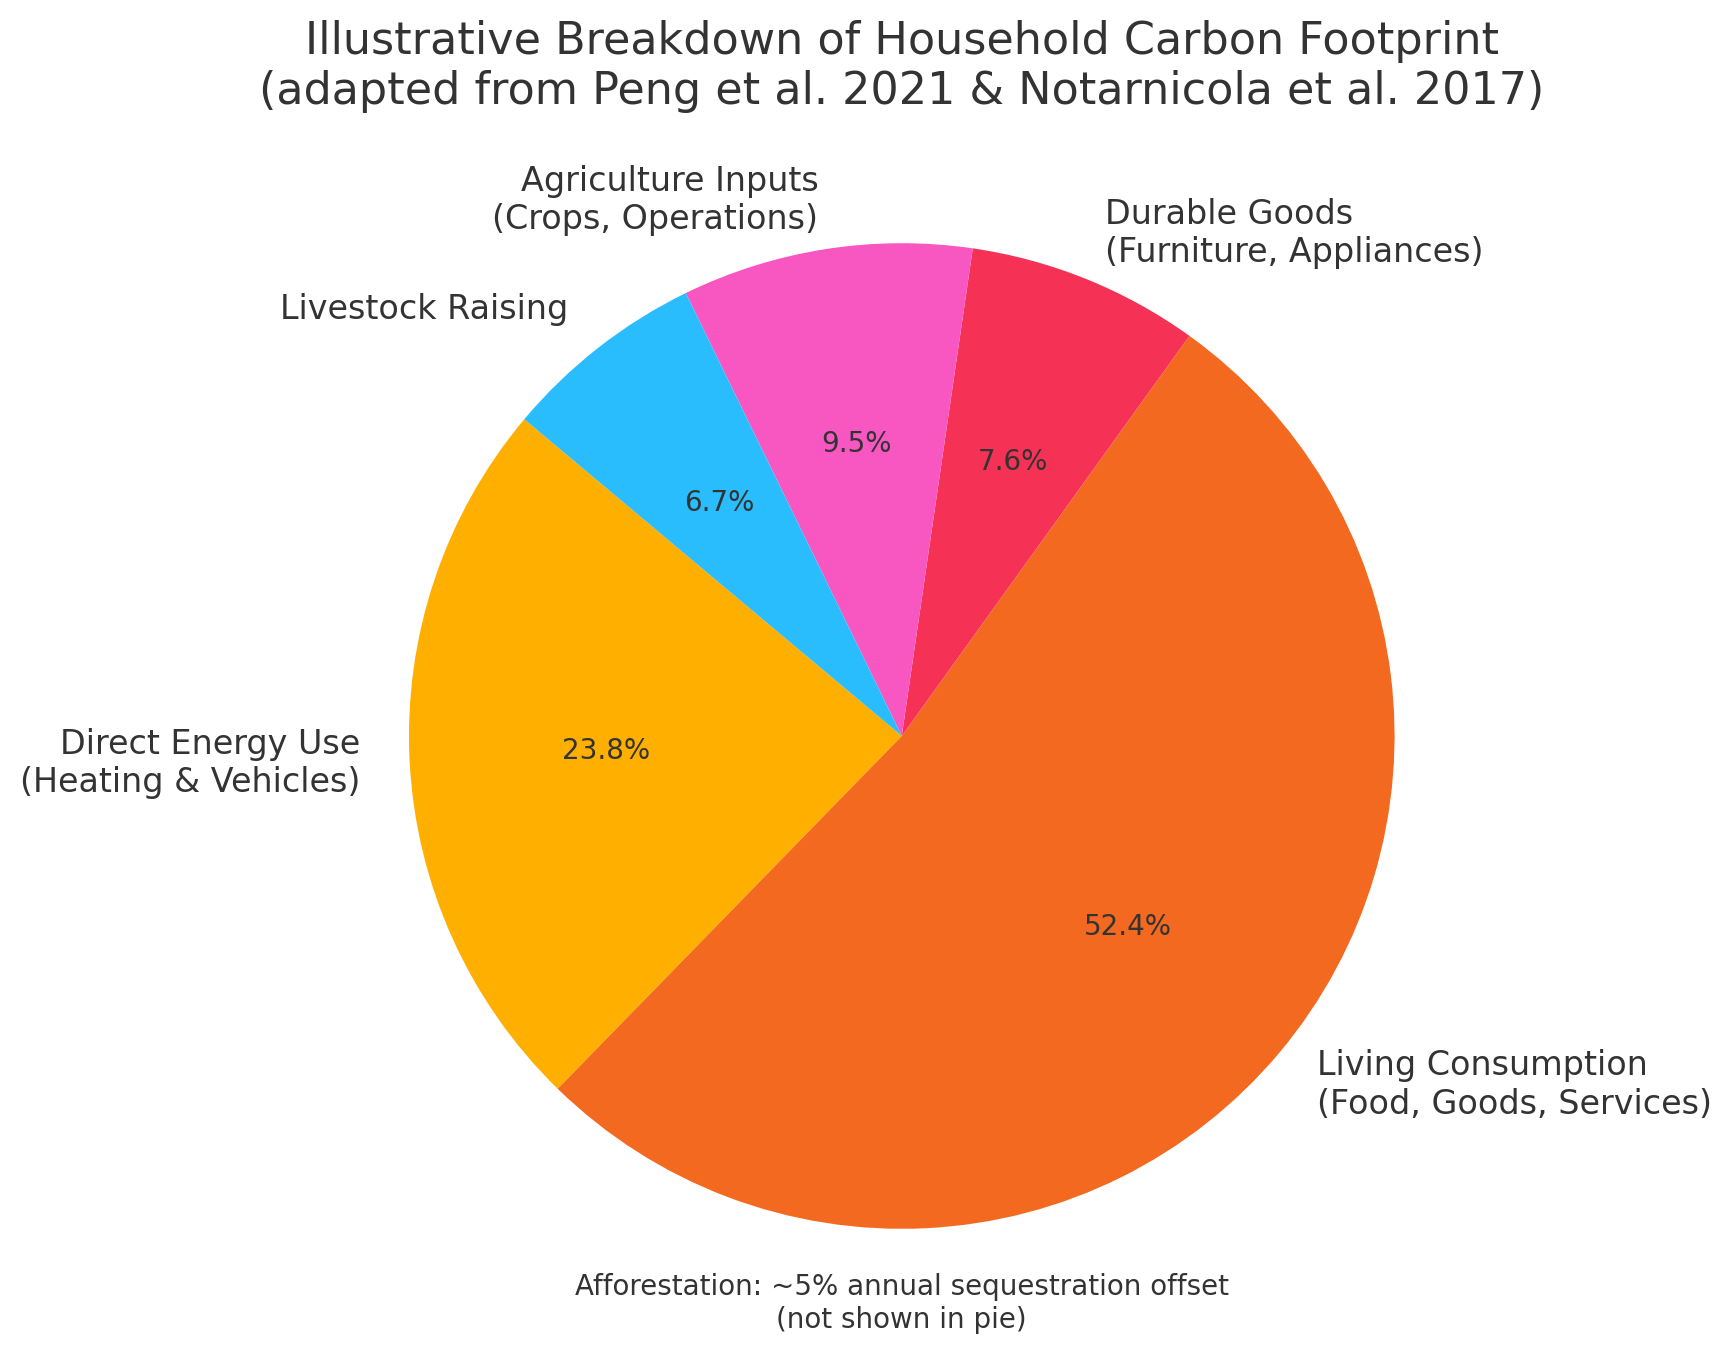
\includegraphics[width=0.68\linewidth]{LCA_pie.png}
\end{center}


\end{frame}

\begin{frame}{Environmentally Extended Input–Output (EEIO) Framework}
\footnotesize
\vspace{-2.5em}
\textbf{Definition:}  
The EEIO model quantifies household carbon footprints by tracing both direct and upstream emissions embedded in goods and services using macroeconomic inter-industry linkages.

\vspace{0.5em}
\textbf{Core Identity:}
\[
\mathbf{X} = (\mathbf{I} - \mathbf{A})^{-1} \cdot \mathbf{F}
\quad
\Rightarrow
\quad
\mathbf{E} = \mathbf{C} \cdot (\mathbf{I} - \mathbf{A})^{-1} \cdot \mathbf{F}
\]

\vspace{0.5em}
\textbf{Components:}
\begin{itemize}
  \item \( \mathbf{A} \): Technical coefficient matrix gives the economic input structure
  \item \( \mathbf{F} \): Final demand vector captures household expenditure
  \item \( \mathbf{C} \): Emission intensity vector (kg CO\textsubscript{2}e / € output)
\end{itemize}

\vspace{0.5em}
\vspace{0.5em}
\textbf{Model Assumptions and Stability:}
\begin{itemize}
  \item Fixed production coefficients (Leontief structure)
  \item No substitution across sectors or inputs
  \item The matrix \( \mathbf{A} \) must satisfy \( \rho(\mathbf{A}) < 1 \) for stability
  \item Empirically: \( \sum_i A_{ij} < 1 \) for all \( j \)
\end{itemize}

\end{frame}

\begin{frame}{EEIO Emissions Decomposition: Tiered Attribution}
\footnotesize
\vspace{-2.0em}
Following Matthews et al. (2008) and Long et al. (2019), household emissions are decomposed into three analytical tiers:

\vspace{0.5em}
\textbf{Tier 1 – Direct Emissions:}
\[
\mathbf{E}_1 = \mathbf{C}_d \cdot \mathbf{F}_d
\quad \text{(e.g., direct fuel use)}
\]

\textbf{Tier 2 – Indirect Energy:}
\[
\mathbf{E}_2 = \mathbf{C}_e \cdot (\mathbf{I} - \mathbf{A})^{-1} \cdot \mathbf{F}_e
\quad \text{(e.g., electricity, heating)}
\]

\textbf{Tier 3 – Indirect Supply Chain:}
\[
\mathbf{E}_3 = \mathbf{C} \cdot \left[(\mathbf{I} - \mathbf{M})(\mathbf{I} - \mathbf{A})\right]^{-1} \cdot \left[(\mathbf{I} - \mathbf{M}) \cdot \mathbf{F} + \mathbf{EX}\right]
\]

\vspace{0.5em}
\textbf{Total Household Footprint:}
\[
\mathbf{E}_{\text{total}} = \mathbf{E}_1 + \mathbf{E}_2 + \mathbf{E}_3
\]

\vspace{0.5em}
\textbf{Note:}  
Import-adjusted tiers ensure that emissions are attributed to domestic demand. Enables national-scale footprint analysis with high coverage.

\end{frame}

\begin{frame}{EEIO Illustration: Method and Aggregate Estimates}
\vspace{-2.0em}
  \footnotesize
\textbf{Methodology:}
\begin{itemize}
  \item Emission intensities \(EF_i\) reflect \( \mathbf{C}(\mathbf{I}-\mathbf{A})^{-1} \), derived from EXIOBASE (via Climatiq.io).
  \item National consumption \(F_{i,c}\) from Eurostat (2021) is multiplied by category-specific \(EF_i\) for each country:
  \[
  E_{i,c} = F_{i,c} \cdot EF_i
  \]
  \end{itemize}

\vspace{0.6em}
\textbf{Total Household Carbon Footprints (2021):}

\begin{table}[h]
\footnotesize
\begin{tabular}{lcc}
\toprule
\textbf{Country} & \textbf{Expenditure (bn €)} & \textbf{Emissions (Mt CO\textsubscript{2}e)} \\
\midrule
France   & 1322.0 & 420.0 \\
Spain    & 747.9  & 227.0 \\
Germany  & 1794.8 & 545.9 \\
\bottomrule
\end{tabular}
\end{table}

\vspace{0.3em}
\footnotesize Source: Eurostat (2021), EXIOBASE (2025); Author’s calculations.
\end{frame}

\begin{frame}{EEIO Illustration: Interpretation of Results}
\small
\vspace{-2.5em}
\textbf{Sectoral Composition of Emissions}
\begin{itemize}
  \item Housing, food, and transport consistently emerge as the most emission-intensive categories.
  \item These three sectors jointly account for over 60\% of total household carbon footprints in France, Spain, and Germany.
\end{itemize}

\vspace{0.6em}
\textbf{Cross-Country Differences}
\begin{itemize}
  \item \textbf{Germany:} Highest absolute emissions, reflecting both higher household expenditure and carbon-intensive energy use.
  \item \textbf{France:} Lower footprint per euro spent, can be attributed to cleaner energy mix and less carbon-intensive consumption.
  \item \textbf{Spain:} Intermediate values, with emissions closely tied to transport and agri-food supply chains.
\end{itemize}


\vspace{0.3em}
\textit{The EEIO framework captures upstream emissions embedded in household consumption, providing a robust basis for cross-country comparison.}
\end{frame}




\end{document}
